\subsection{Nodo di controllo}

\subsubsection{Artificial Potential Field}
Per poter utilizzare tale tipologia di controllo bisogna calcolare il \textit{goal} dinamicamente, cioè calcolare l'intersezione tra la retta e il cerchio di raggio r. Ricodiamo che le coordinate $(x_r,y_r)$ coincidono con quelle del rover. Impostando il sistema:

\begin{equation} 
\begin{cases}

    (x-x_r)^2+(y-y_r)^2=r^2
   \\
    y=mx+q 
  \end{cases} 
\end{equation}
si sostituisce la seconda equazione nella prima
\begin{equation}
(x-x_r)^2+(mx+q-y_r)^2=r^2
\end{equation}

\begin{equation}
x^2+x_r^2-2xx_r+m^2x^2+q^2+y_r^2+2mxq-2mqy_r-2mxy_r-r^2=0
\end{equation}

\begin{equation}
\underbrace{(1+m^2)}_\text{a}x^2+\underbrace{(2mq-2x_r-2my_r)}_\text{b}x+\underbrace{(x_r^2+q^2+y_r^2-2qy_r-r^2)}_\text{c}=0
\end{equation}
Definiamo $\Delta=b^2-4ac=(2mq-2x_r-2my_r)^2-4(1+m^2)(x_r^2+q^2+y_r^2-2qy_r-r^2)$. \\Se:
\begin{itemize}
    \item $\Delta>0$ si hanno due soluzioni
        \begin{equation}
        x_1=\frac{-(2mq-2x_r-2my_r)+\sqrt{2mq-2x_r-2my_r)^2-4(1+m^2)(x_r^2+q^2+y_r^2-2qy_r-r^2)}}{2(1+m^2)}
        \end{equation}
        \\
        \begin{equation}
        x_2=\frac{-(2mq-2x_r-2my_r)-\sqrt{2mq-2x_r-2my_r)^2-4(1+m^2)(x_r^2+q^2+y_r^2-2qy_r-r^2)}}{2(1+m^2)}
        \end{equation}
        Di queste due soluzioni si sceglie quella più lontana rispetto alla posizione dell'ArUco.
    \item $\Delta=0$ si ha una sola soluzione
    \begin{equation}
        x_d=\frac{-(2mq-2x_r-2my_r)}{2(1+m^2)}
        \end{equation}
    \item $\Delta<0$ non si hanno soluzioni, per cui usiamo la proiezione ortogonale tra la retta $y=mx+q$ e la retta passante per le coordinate $(x_r, y_r)$ del rover.
\end{itemize}
Il punto così ottenuto è il $\boldsymbol{q_G}$ della \autoref{APF}.
Si applicano quindi le formule viste in tale sottosezione con i seguenti parametri

\begin{table} [H]
    \centering
    \begin{tabular}{|cc|}
    \hline
        Parametro & Valore usato \\  \hline
        $k_a$ &      \\  \hline
        $k_r$ &    \\  \hline
        $\delta$ &    \\  \hline
        $\delta_0$ &    \\  \hline
    \end{tabular}
\end{table}

\subsection{Nodo di visione}
Gli obiettivi del nodo visione sono:
\begin{enumerate}
  \item riconoscere nell'immagine i markers ArUco;
  \item localizzarli nella mappa;
  \item ricavare l'id del marker e quindi il coefficiente angolare della retta a cui il robot dovrà convergere.
\end{enumerate}
  Per quanto riguarda il primo punto, la libreria OpenCV (\cite{opencv_library}) mette a disposizione un modulo che permette di ricavare la posizione degli angoli del 
  marker e di ricavare l'id associato. \\
  Riguardo il secondo punto, supponendo di conoscere la matrice di calibrazione $K$ della camera (\cite{multiple_view}) e la posizione dell'ArUco in coordinate omogenee 
  $p_w = (X \: Y \: Z \: 1 )^T$, se definiamo il punto immagine come in coordinate pixel $ p_c =  (u \: v \: 1)^T$ si ottiene 
    \begin{equation}
    p_c \propto K [R | \boldsymbol{t}] p_w  \Rightarrow
     \begin{bmatrix}
           u \\
           v \\
           1
        \end{bmatrix}
         \propto 
         \begin{bmatrix}
           f_x & \sigma & c_x \\
           0 & f_y & c_y \\
           0 & 0 & 1 
         \end{bmatrix}
         \begin{bmatrix}
           r_{11} & r_{12} & r_{13} & t_1 \\
           r_{21} & r_{22} & r_{23} & t_2 \\
           r_{31} & r_{32} & r_{33} & t_3 
         \end{bmatrix}
         \begin{bmatrix}
           X \\
           Y \\
           Z \\
           1
    \end{bmatrix}
  \end{equation}
  con R matrice di rotazione e $ \boldsymbol{t}$ vettore che indica la traslazione tra la camera e il marker; calcolando questi due elementi si può ricavare la 
  posa del target in terna camera. Per risolvere questo problema sono stati realizzati vari algoritmi, i queli possono essere richiamati dalla funzione 
  \texttt{solve\_PnP()} della libreria. \\
  A partire quindi dalla posa del marker rispetto a camera e dalla posa della camera in terna fissa si può ottenere la posizione in terna fissa del marker $(x_A, y_A)$.\\
  Infine, l'id del marker permette di ricavare il coefficiente angolare $m_{id}$. Supponendo che il marker giaccia sulla retta con tale $m$, si ricava il 
  parametro mancante $q$ come $ q = y_A - m_{id}x_A$.
\subsection{SMC}
Come visto nella \autoref{SMC_Theory} per definire un controllo SMC si ha bisogno di una funzione $u$ che nel nostro caso è stata scelta pari a: 
\begin{equation}
        u_i=-\rho_{i}sign(\sigma_i)\: \: \: \: \: \: \: \:i=1,2
\end{equation}
con $\rho_i>0 \: \: \:i=1,2$. \\
Definiti poi gli errori 
\begin{equation}
\begin{cases}
    e_1=x_d-x 
   \\
   e_2=y_d-y
   \\
   e_3=\theta_d-\theta
\end{cases} 
\end{equation}
le superfici di sliding sono
\begin{equation}
       \sigma_1=e_1 \ \ \ \ \ \ \ \ \sigma_2=e_3-\arcsin(f(e_2))
\end{equation} 
dove $f(e_2)=-\min({\delta_1|e_2|^{-1},\ \delta_2})$ con $\delta_1 \in (0,1)$, $\delta_2>0$.\\ Per ottenere i guadagni $\rho_1$ e $\rho_2$ si calcolano i paramtri  $r_1$, $r_2$ e $r_3$ in tale modo
\begin{equation}
        r_1= \max\left\{\frac{\delta_1+d_1-d_3)\sqrt{1-\delta_1^{2}}}{1+d_3-d_1}v_{max}, \frac{(1+d_2)(\omega_{max}+\rho_2) \frac{\rho_1}{\rho_2}+d_2v_{max}}{1-d_1}\right\}
\end{equation}
\begin{equation}
        r_2= \min\left\{\frac{\delta_1-d_3\sqrt{1-\delta_1^{2}}}{d_3}v_{min}, \frac{\delta_1}{d_3}-v_{max}\sqrt{1-\delta_1^{2}}\right\}
\end{equation}
\begin{equation}
        r_3= \frac{\delta_1-d_3\sqrt{1-\delta_1^{2}}+\delta_2v_{max}+\delta_1v_{min}}{(1-d_2\sqrt{1-\delta_1^{2}}}
\end{equation}
e si sceglie $r_1<\rho_1<r_2$,\ \ $r_3<\rho_2$. Con tale scelta la dinamica dell'errore converge asintoticamente all'insieme
\begin{equation}
        D=\left\{(e_1,e_2,e_3) \in \mathbb{R}: e_1=0, \ \  |e_2|\le\delta_2^{-1}C, \ \ |e_3|\le \arcsin{(C)} \right\}
\end{equation}
con $C=\frac{d_3(\rho_1+v_{max}\sqrt{1-\delta_1^{2}})}{v_{min}}$.
\begin{figure} [H]
    \centering
    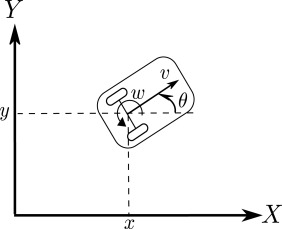
\includegraphics[width=0.5\linewidth]{img/SMC.jpg}
    \caption{Sliding Mode Control}
    \label{fig:SMC}
\end{figure}